%% Run with the following three lines uncommented for article pdf and comment for presentation pdf
%\documentclass[a4paper]{article}
%\usepackage{beamerarticle}
%\mode<article>{\usepackage{fullpage}}
%%

%% Run with the following line uncommented for presentation pdf and commented for article pdf
\documentclass[ignorenonframetext]{beamer}
%\documentclass[ignorenonframetext,draft]{beamer}
\setbeamertemplate{navigation symbols}{}
%%

\usepackage{ esint } % for multi-dimensional integrals
% \usepackage{movie15}
\usepackage{hyperref}
\usepackage{pgf}
\usepackage{subfigure}
% \usepackage{movie15}
\mode<presentation>
%{
%\usetheme{madrid}
%\usetheme{frankfurt}
    \usetheme{Copenhagen}
\useoutertheme{infolines} % this makes only immediate navigation at top of slide
%\setfootline{\insertshortinstitute, \insertshortdate
%\hfill slide \insertframenumber/\inserttotalframenumber}
%}
\setbeamertemplate{headline}{}

\title[SciPy 2014]{Perceptions of Matplotlib colormaps}

\author{Kristen M. Thyng}
\date{July 10, 2014}
\institute[Texas A\&M]{Texas A\&M University}
    
% In case you want to use a logo (e.g. in png format): 
% \pgfdeclareimage[height=1.0cm]{university-logo}{figures/logo_tamu} 
% \logo{\pgfuseimage{university-logo}}

% \input{../../LatexFiles/macros}

% % Extra slides don't contribute to slide number at bottom right
% \input{appendixnumberbeamer.sty}

\AtBeginSection[]
{
    \begin{frame}
        \frametitle{Outline}
        \tableofcontents[currentsection]
    \end{frame}
}

\begin{document}
\begin{frame}
    \titlepage
\end{frame}


% \begin{frame}
%   \frametitle{Outline}
%   \tableofcontents
% \end{frame}


%%%  %%%

\section{}

\begin{frame}[t]\frametitle{CIELAB Color Model}
    \begin{figure}[htbp]
        \centering
        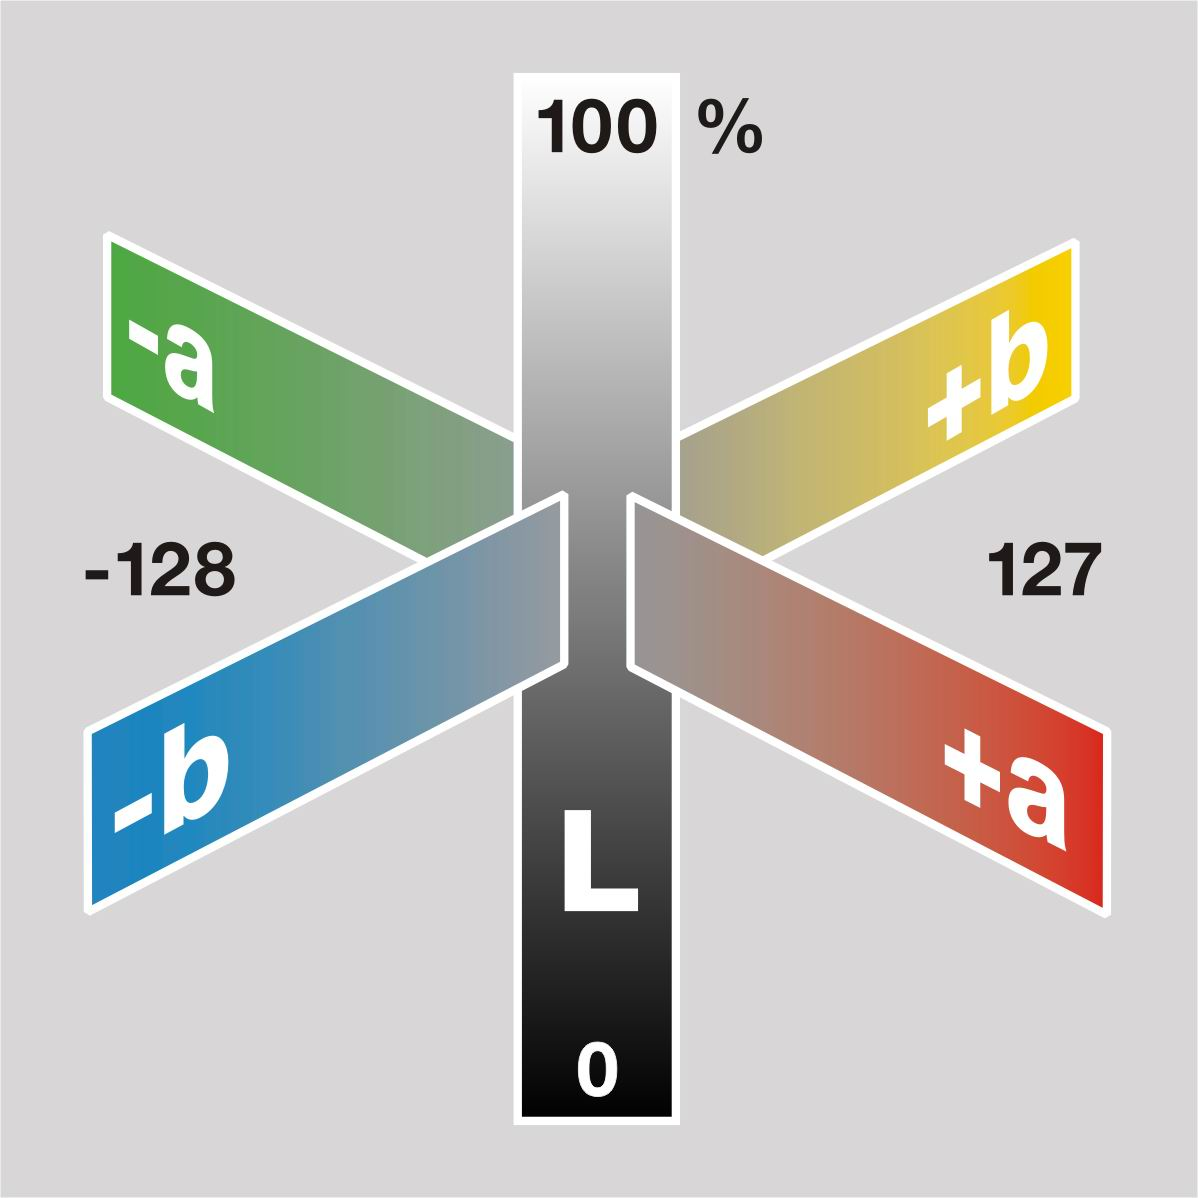
\includegraphics[width=0.55\textwidth]{figures/Cielab.jpg}
    \end{figure}
    \tiny{http://eschicleypega.blogspot.com}
\end{frame}

\begin{frame}[t]\frametitle{Lightness of matplotlib Colormaps}
    \begin{figure}[htbp]
        \centering
        \only<1>{
        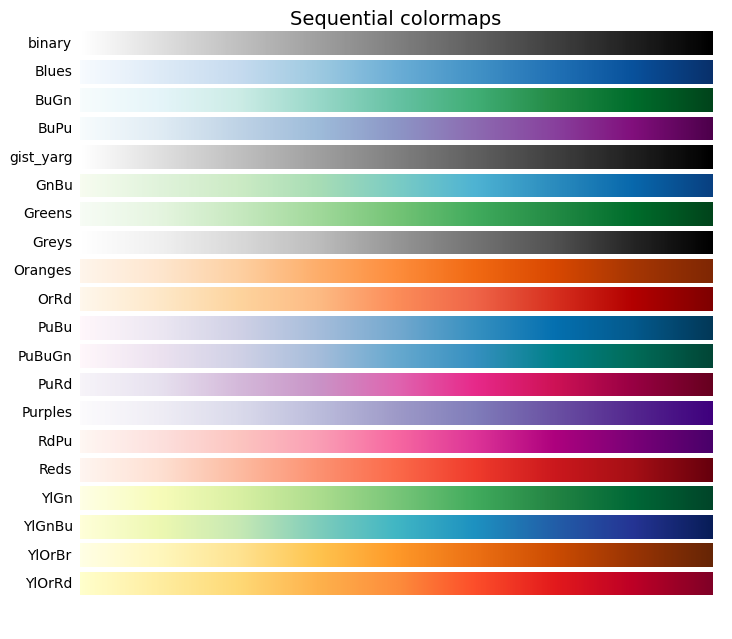
\includegraphics[width=0.45\textwidth]{figures/seq}
        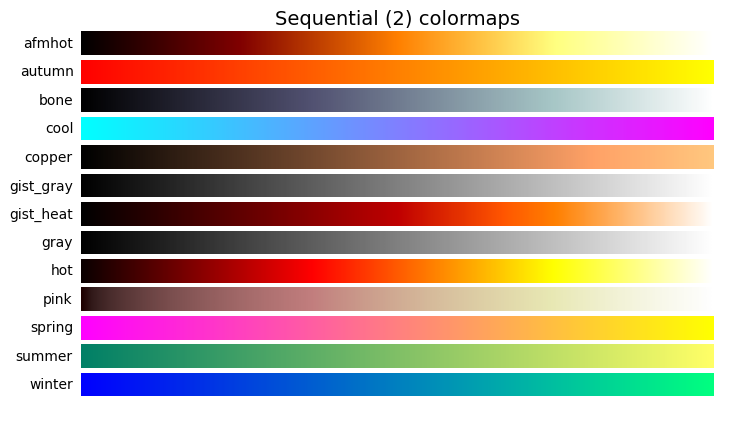
\includegraphics[width=0.45\textwidth]{figures/seq2}}
        \only<2>{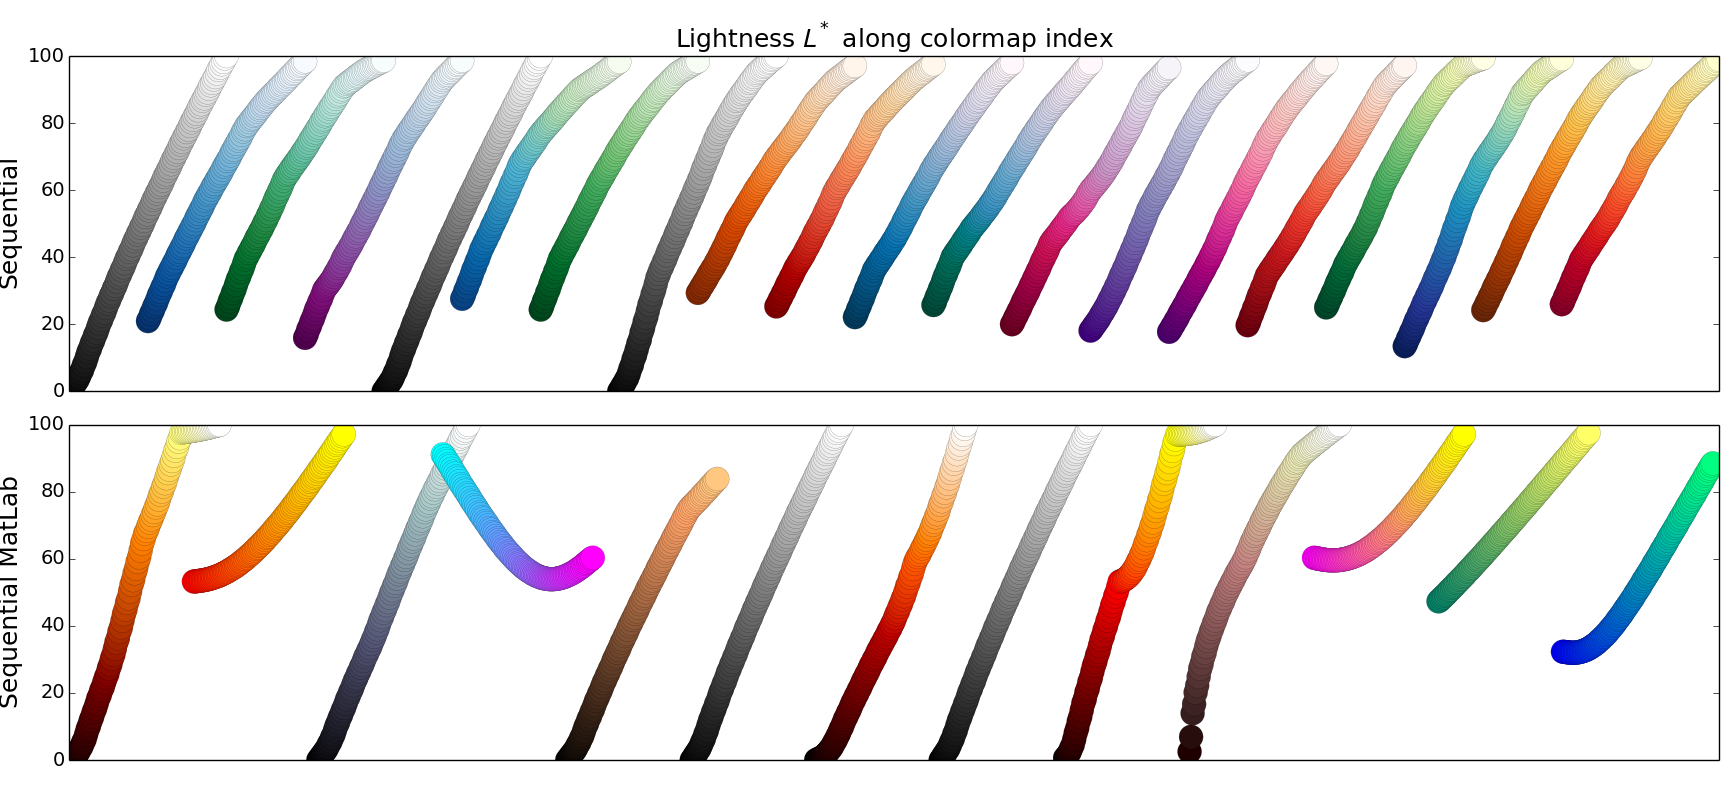
\includegraphics[width=\textwidth]{figures/lightness-sequential}}
    \end{figure}
    \only<1>{
    \vskip8ex
    \tiny{http://matplotlib.org/examples/color/colormaps\_reference.html}}
\end{frame}

\begin{frame}[t]\frametitle{Lightness of matplotlib Colormaps}
    \begin{figure}[htbp]
        \centering
        \only<1>{
        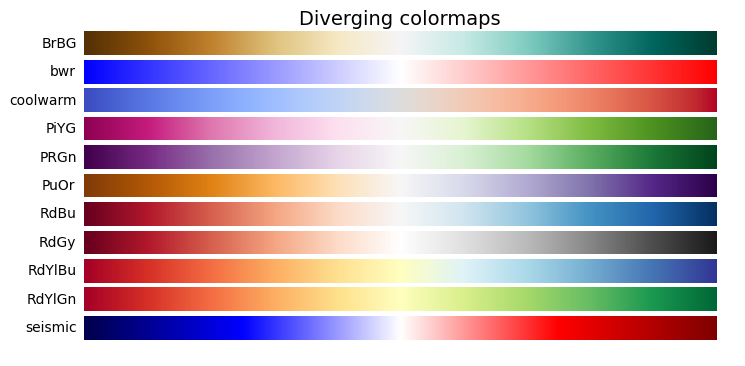
\includegraphics[width=0.45\textwidth]{figures/div}
        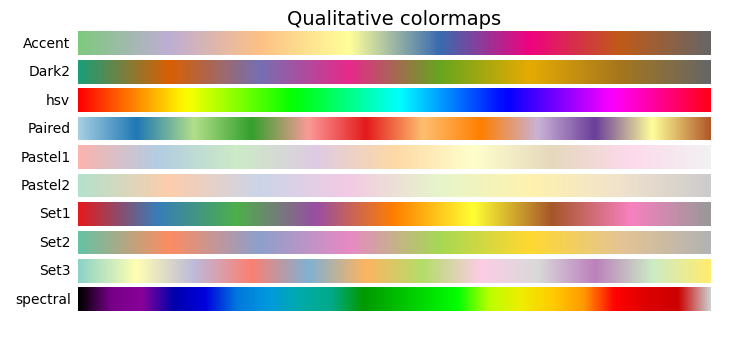
\includegraphics[width=0.45\textwidth]{figures/qual}\\
        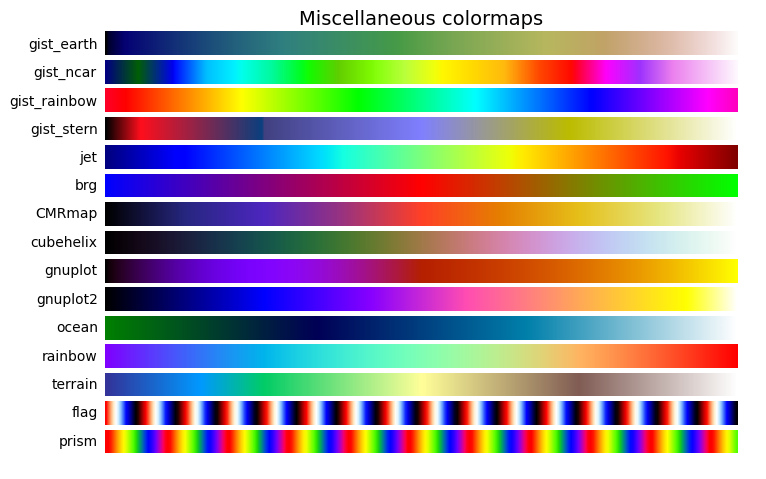
\includegraphics[width=0.45\textwidth]{figures/misc}}
        \only<2>{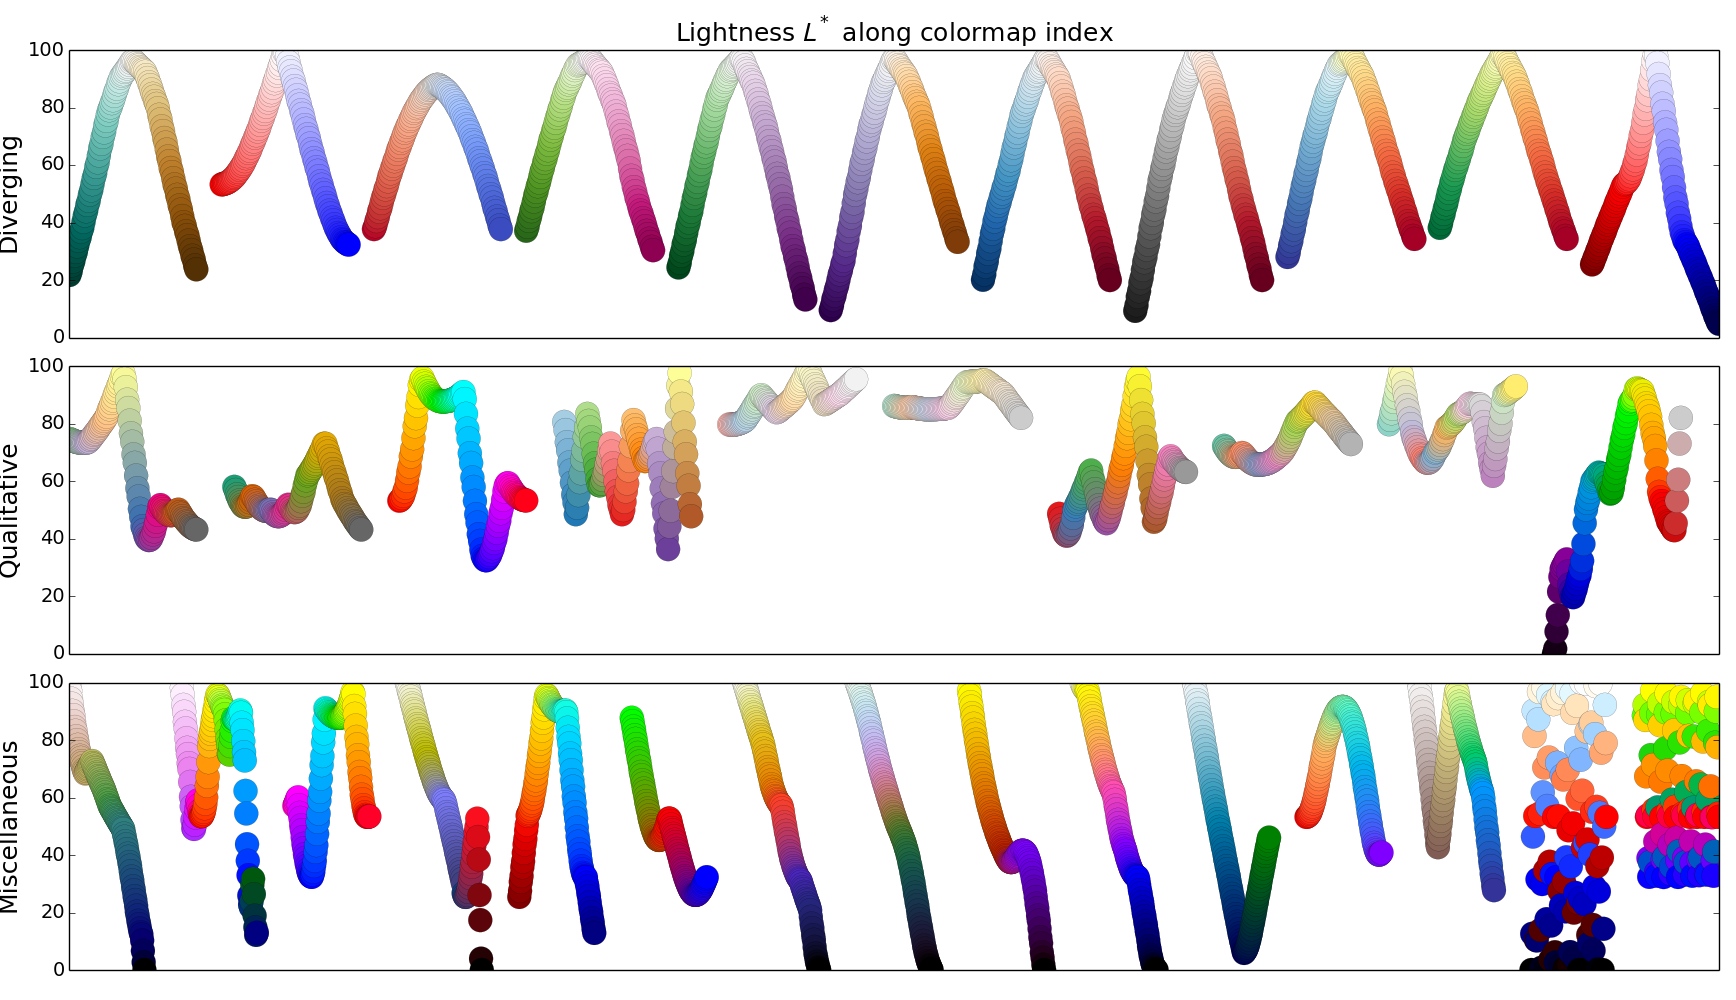
\includegraphics[width=\textwidth]{figures/lightness-rest}}
    \end{figure}
    \only<1>{
    \tiny{http://matplotlib.org/examples/color/colormaps\_reference.html}}
\end{frame}

\begin{frame}[t]\frametitle{Perceived Lightness: Weber-Fechner Law}
    \vskip-2ex
    \begin{figure}[htbp]
        \centering
        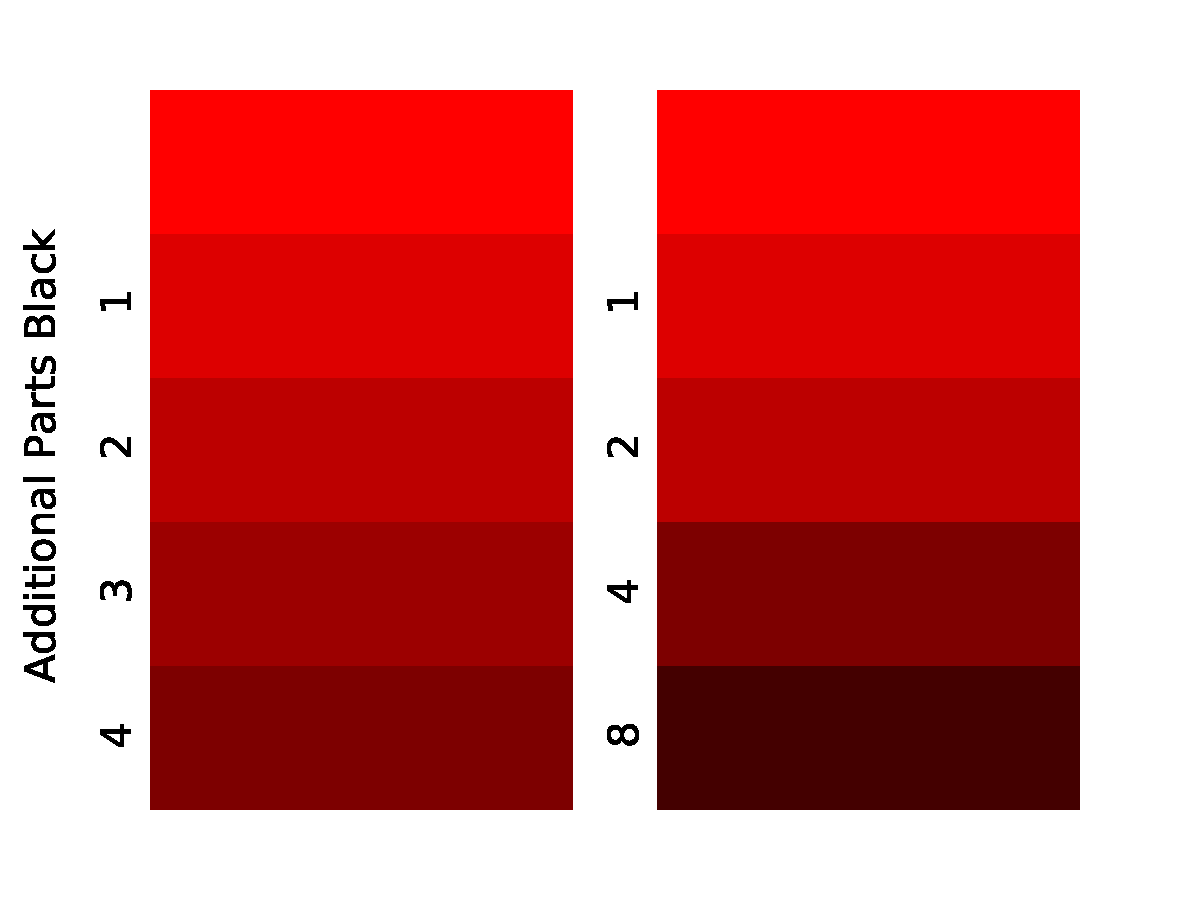
\includegraphics[width=0.8\textwidth]{figures/albers.pdf}
    \end{figure}
    \vskip-2ex
    \tiny{Albers, J. (1975). Interaction of color. Yale University Press.}
\end{frame}

\begin{frame}[t]\frametitle{Improvement to Binary Colormap?}
    \begin{figure}[htbp]
        \centering
        \only<1>{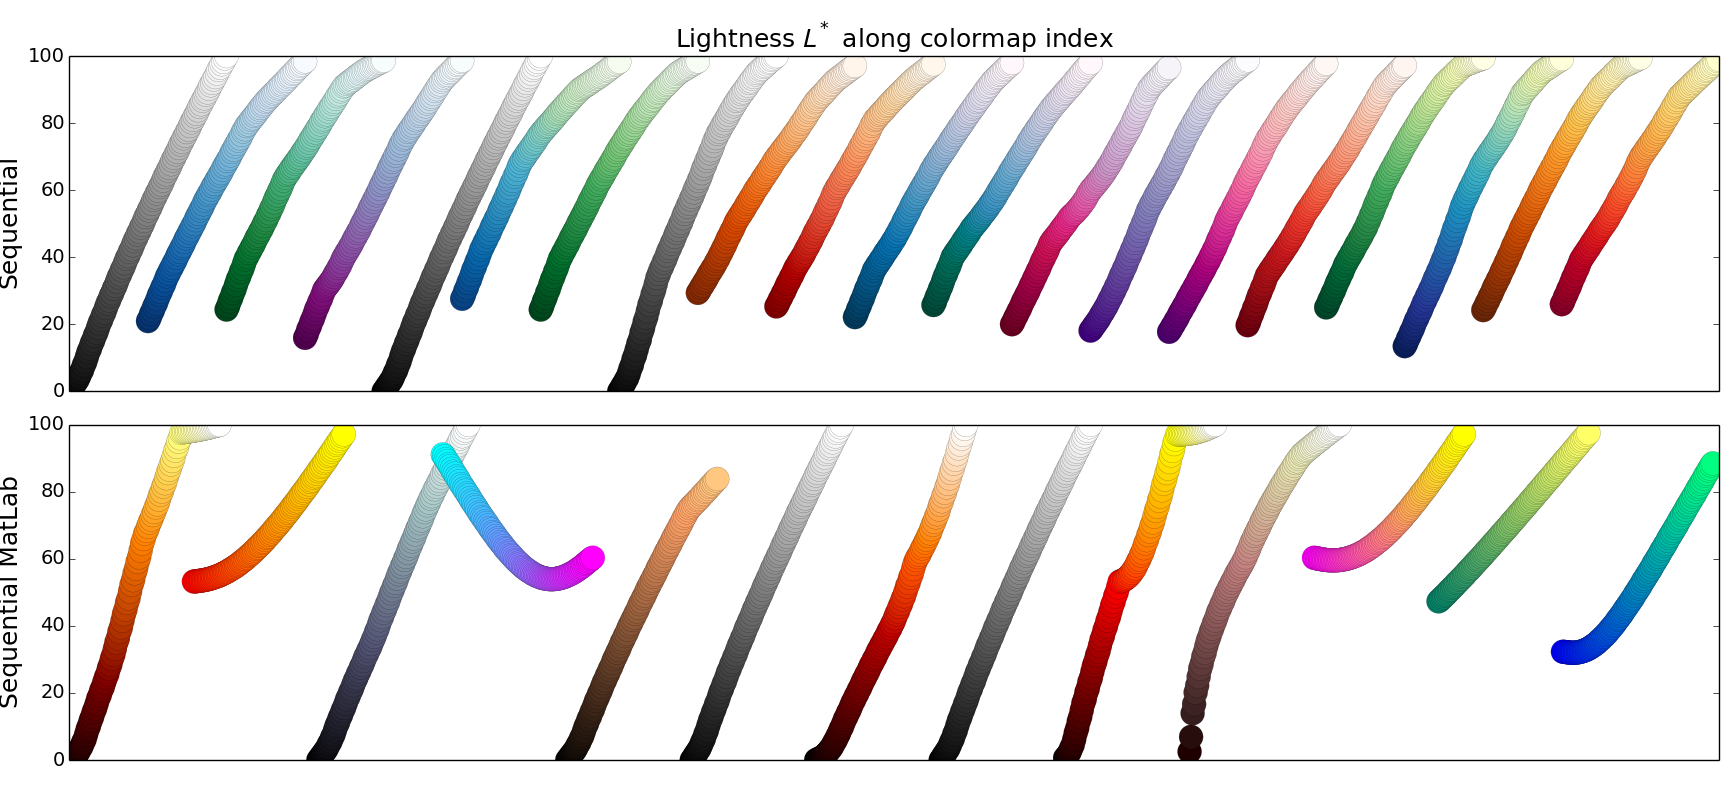
\includegraphics[width=\textwidth]{figures/lightness-sequential}}
        \only<2>{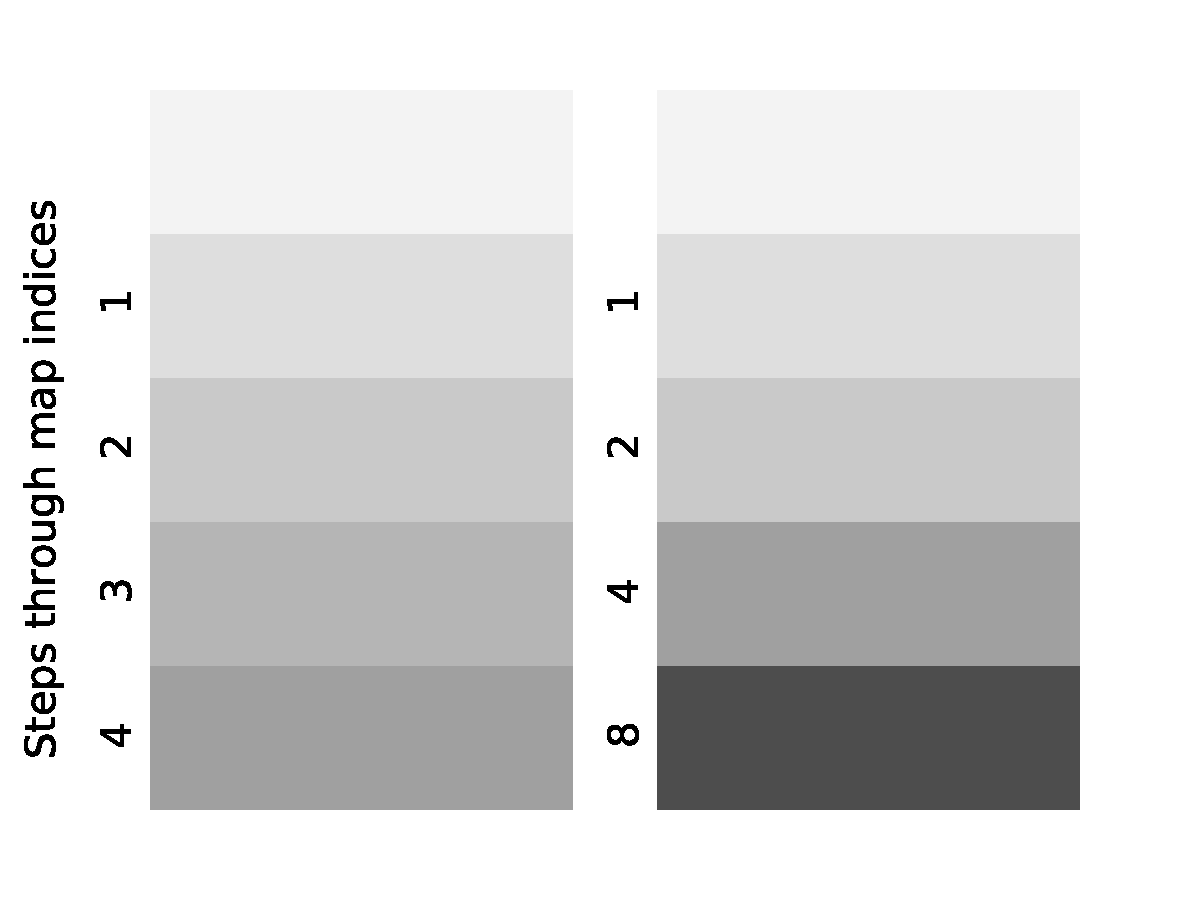
\includegraphics[width=0.8\textwidth]{figures/albers-bw}}
    \end{figure}
\end{frame}

% \begin{frame}[t]\frametitle{Harmonic Colors}
    
% MAYBE DO THIS TO INCLUDE HUE

% \end{frame}

\begin{frame}[t]\frametitle{Printing to Grey Scale}
% MATTERS ESPECIALLY FOR DIVERGING COLORMAPS AS LONG AS LIGHTNESS IS MONOTONICALLY INCREASING IN SEQUENTIAL COLORMAP
    
MANY WAYS TO DO THIS - introduce a few ways
What to be aware of? What is best? There are many algorithms but probably best is just to be monotonically increasing in luminance

\end{frame}

\begin{frame}[t]\frametitle{matplotlib Colormaps in Grey Scale}
    \begin{figure}[htbp]
        \centering
        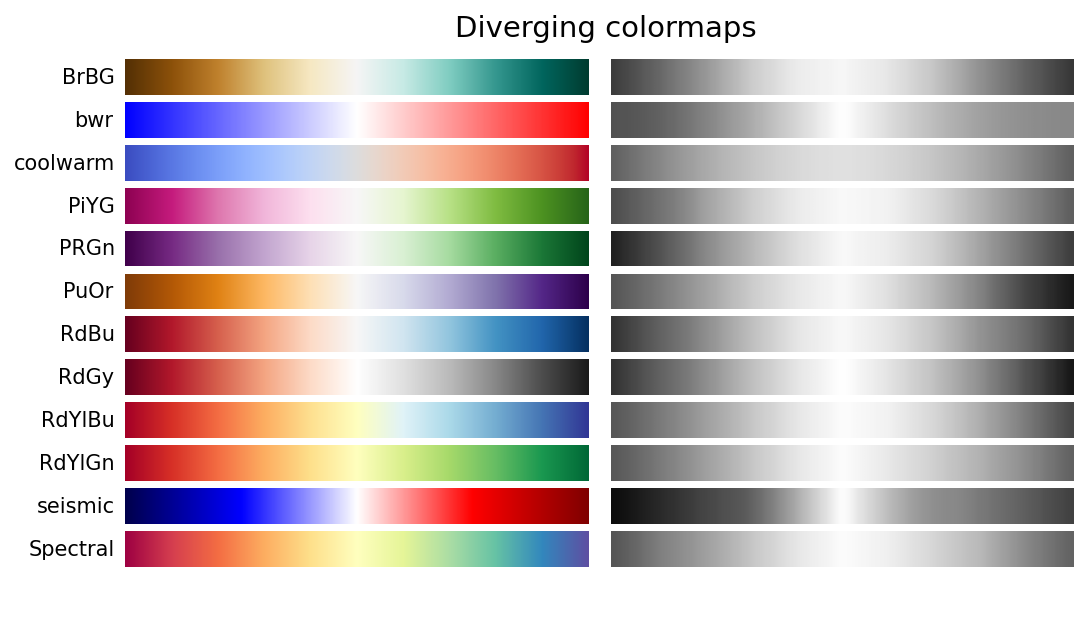
\includegraphics[width=\textwidth]{figures/bwDiverging}
    \end{figure}
\end{frame}
\begin{frame}[t,noframenumbering]\frametitle{matplotlib Colormaps in Grey Scale}
    \begin{figure}[htbp]
        \centering
        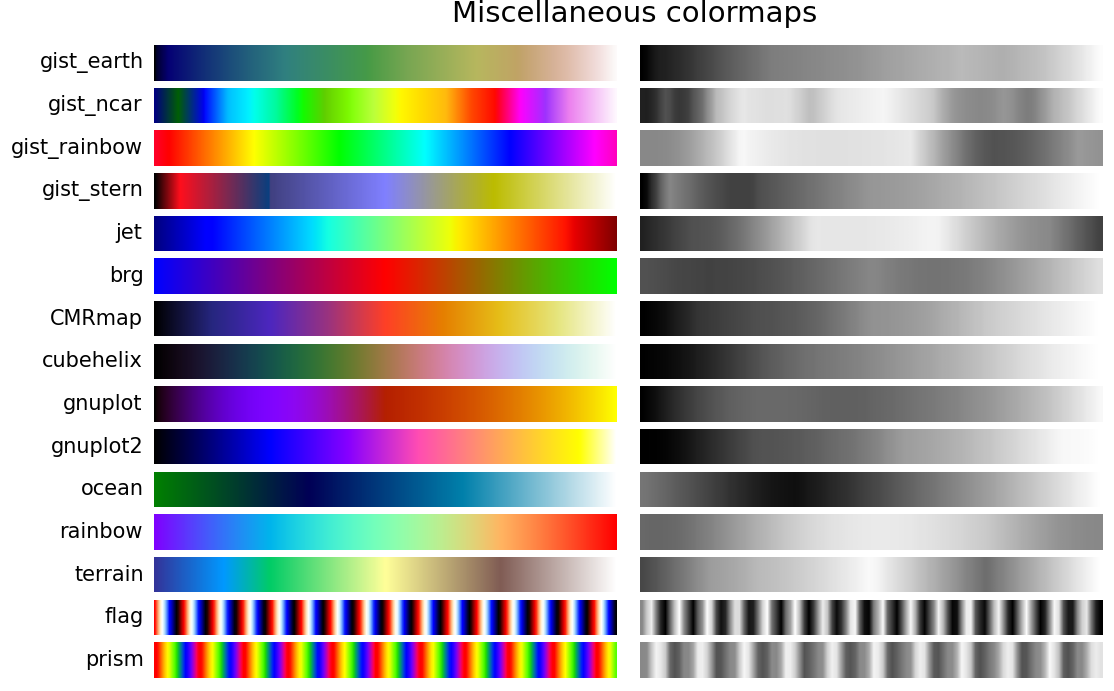
\includegraphics[width=\textwidth]{figures/bwMiscellaneous}
    \end{figure}
\end{frame}
\begin{frame}[t,noframenumbering]\frametitle{matplotlib Colormaps in Grey Scale}
    \begin{figure}[htbp]
        \centering
        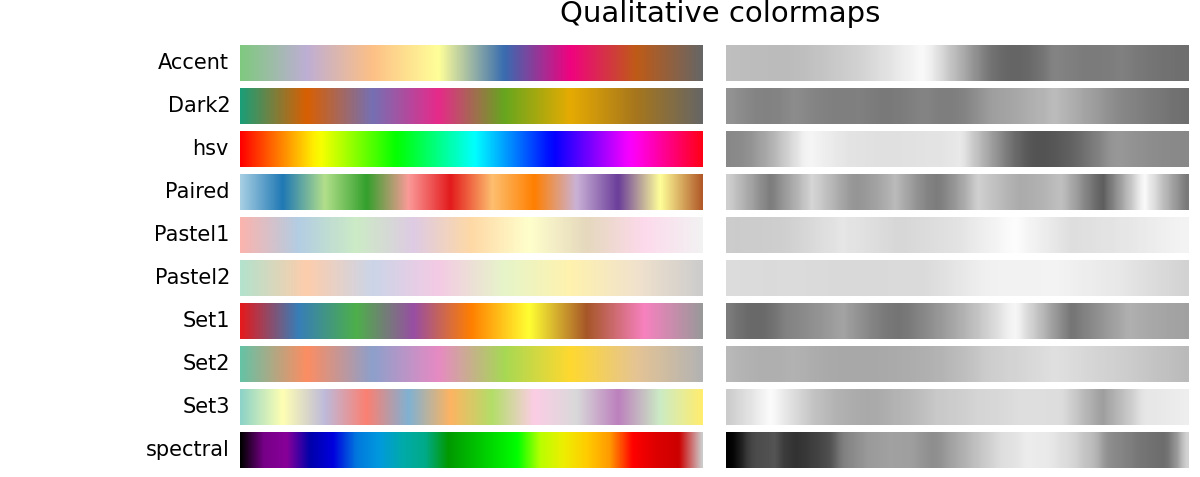
\includegraphics[width=\textwidth]{figures/bwQualitative}
    \end{figure}
\end{frame}
\begin{frame}[t,noframenumbering]\frametitle{matplotlib Colormaps in Grey Scale}
    \begin{figure}[htbp]
        \centering
        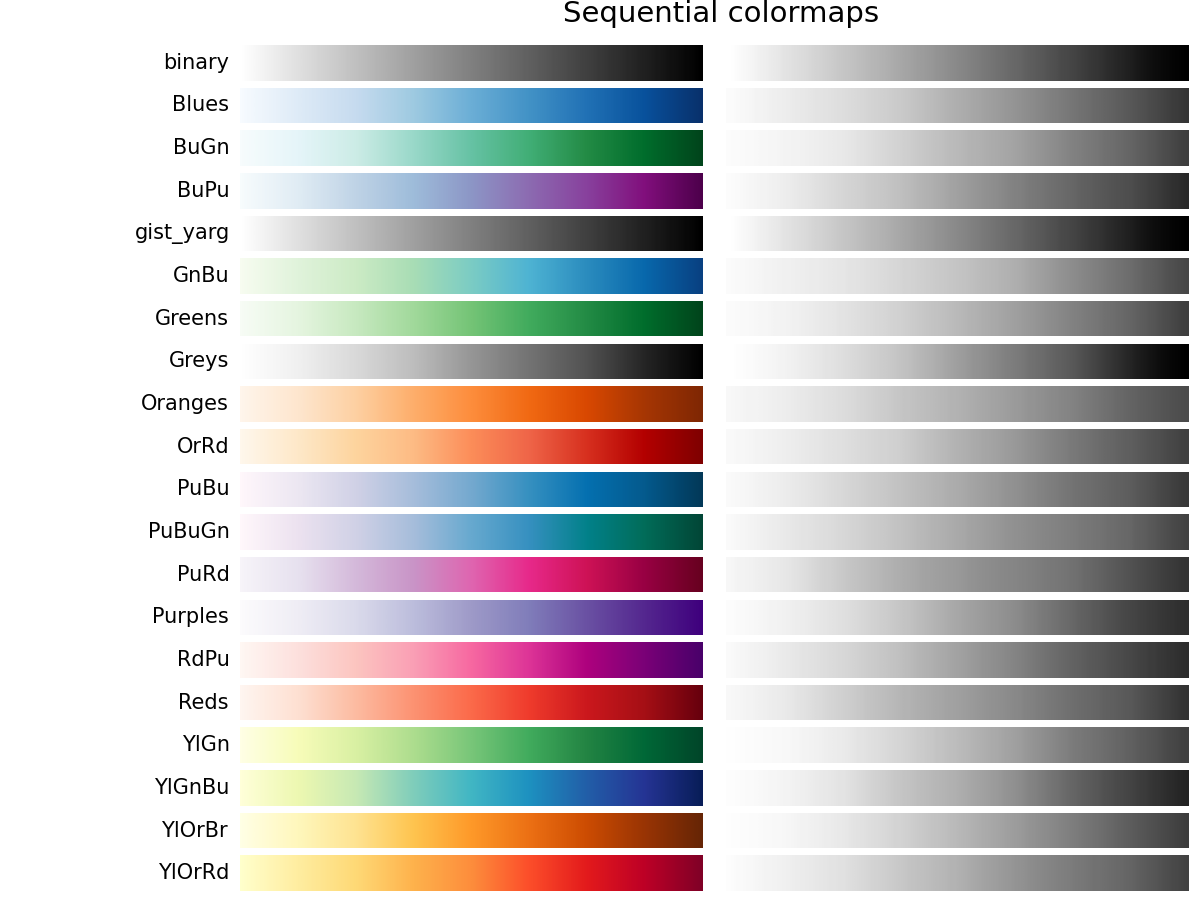
\includegraphics[width=0.7\textwidth]{figures/bwSequential}
    \end{figure}
\end{frame}
\begin{frame}[t,noframenumbering]\frametitle{matplotlib Colormaps in Grey Scale}
    \begin{figure}[htbp]
        \centering
        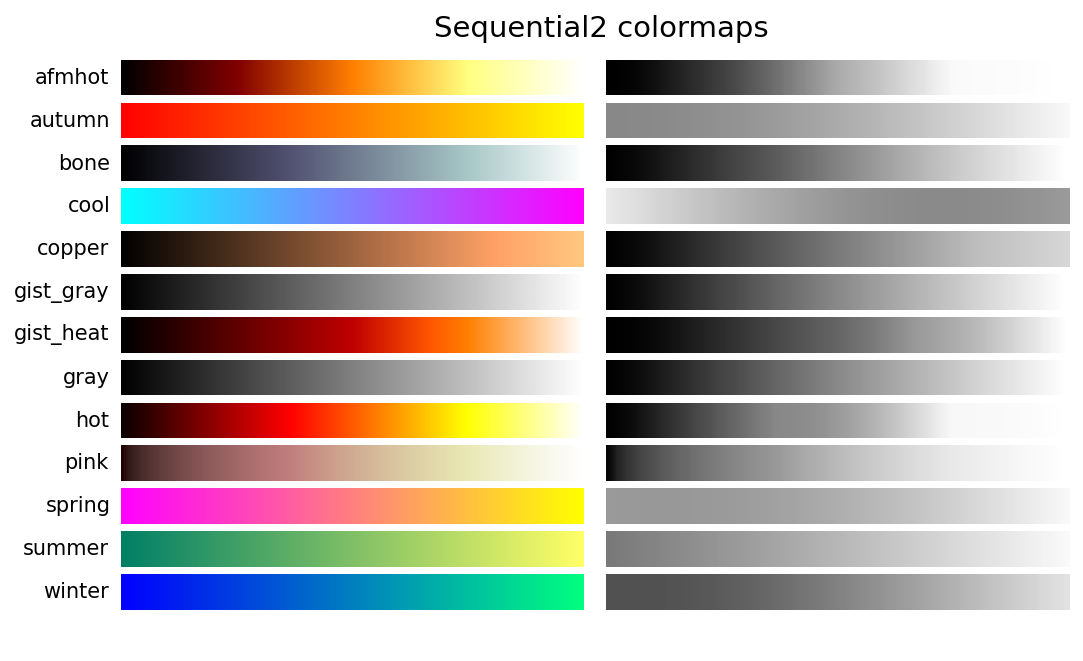
\includegraphics[width=\textwidth]{figures/bwSequential2}
    \end{figure}
\end{frame}

\begin{frame}[t]\frametitle{Color Blindness}
    Protanopia (2\% male population, half mild form)
    \begin{figure}[htbp]
        \centering
        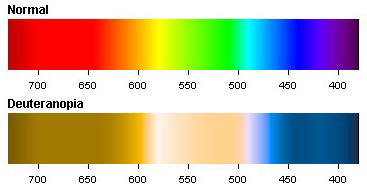
\includegraphics[width=0.43\textwidth]{figures/deuteranopia-color-spectrum}
    \end{figure}
    Deuteranopia (6\% male population, mostly mild form)
    \begin{figure}[htbp]
        \centering
        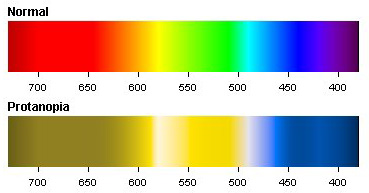
\includegraphics[width=0.43\textwidth]{figures/Protanopia-Color-Spectrum}
    \end{figure}
    \vskip-1ex
    \tiny{http://www.color-blindness.com}
\end{frame}
\begin{frame}[t]\frametitle{Color Blindness}
    \begin{figure}[htbp]
        \centering
        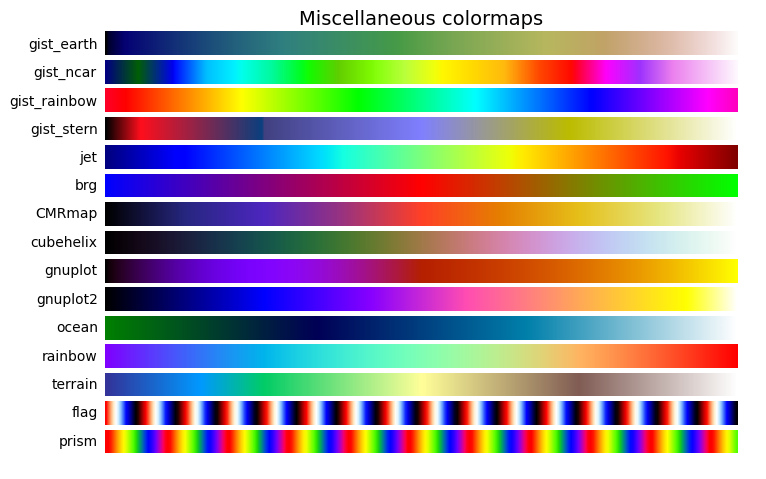
\includegraphics[width=0.49\textwidth]{figures/misc}
        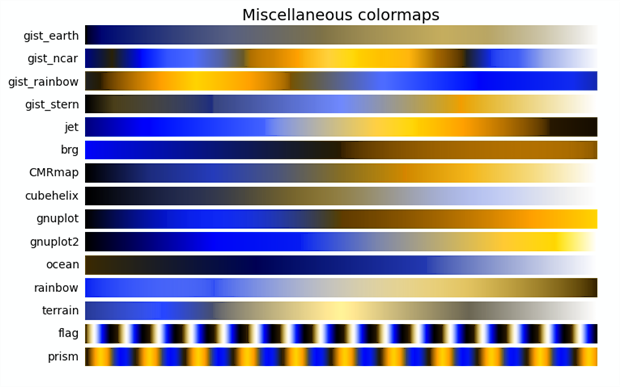
\includegraphics[width=0.49\textwidth]{figures/misc_deuteranopia}
    \end{figure}
    \vskip16ex
    \tiny{http://aspnetresources.com/tools/colorBlindness}
\end{frame}
\begin{frame}[t]\frametitle{Color Blindness}
    \begin{figure}[htbp]
        \centering
        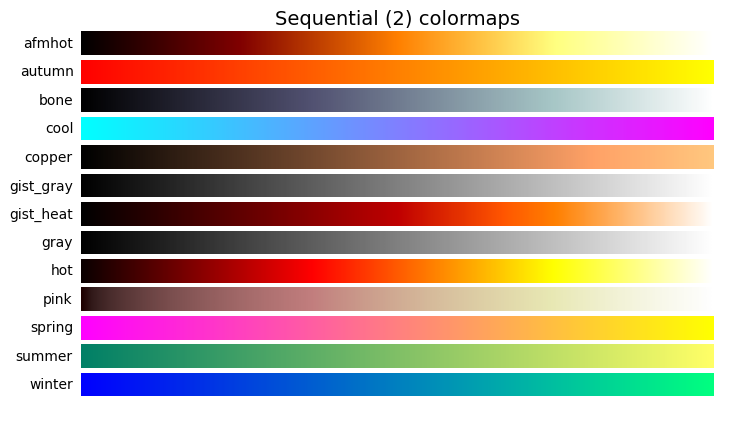
\includegraphics[width=0.49\textwidth]{figures/seq2}
        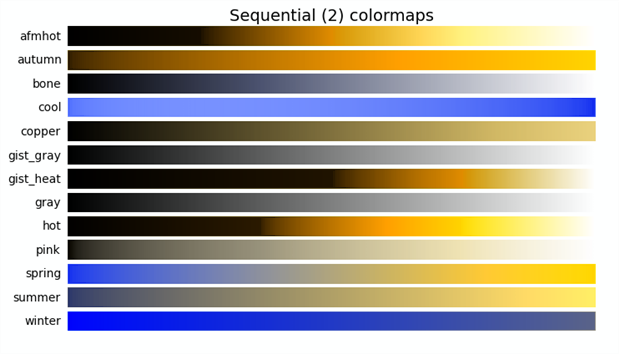
\includegraphics[width=0.49\textwidth]{figures/seq2_deuteranopia}
    \end{figure}
    \vskip18ex
    \tiny{http://aspnetresources.com/tools/colorBlindness}
\end{frame}
\begin{frame}[t]\frametitle{Color Blindness}
    \begin{figure}[htbp]
        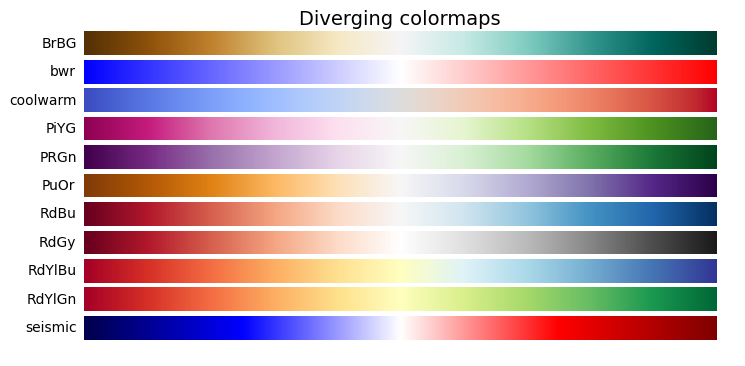
\includegraphics[width=0.49\textwidth]{figures/div}
        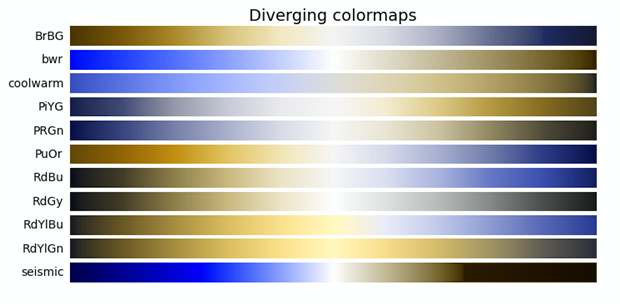
\includegraphics[width=0.49\textwidth]{figures/div_deuteranopia}
    \end{figure}
    \vskip22ex
    \tiny{http://aspnetresources.com/tools/colorBlindness}
\end{frame}
\begin{frame}[t]\frametitle{Color Blindness}
    \begin{figure}[htbp]
        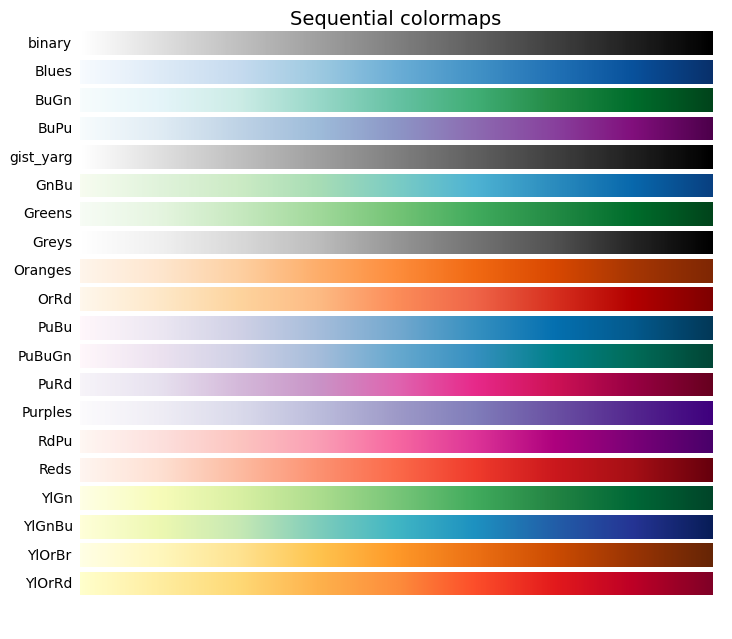
\includegraphics[width=0.49\textwidth]{figures/seq}
        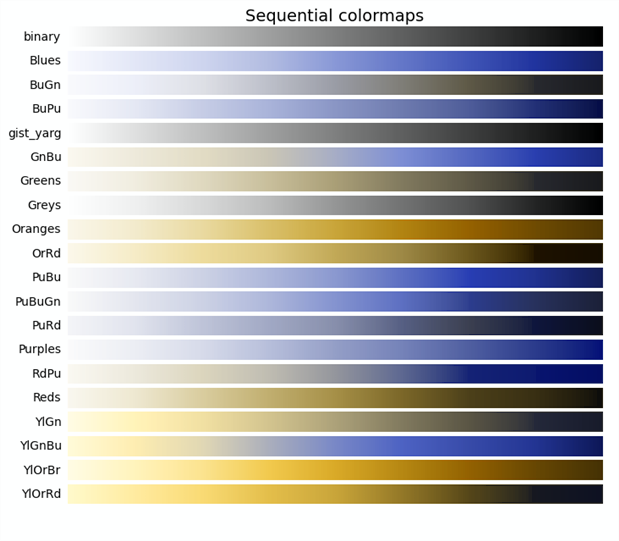
\includegraphics[width=0.49\textwidth]{figures/seq_deuteranopia}
    \end{figure}
    \vskip8ex
    \tiny{http://aspnetresources.com/tools/colorBlindness}
\end{frame}

\begin{frame}[t]\frametitle{Recommendations}
\begin{itemize}
    \item Best colormap depends on application, but for form information, perceptual colormaps are best
    \item Colormap for best lightness perception, hue combination, printing to grey, and color blindness? FILL IN
\end{itemize}
\end{frame}

\begin{frame}[t]\frametitle{Resources}
\begin{itemize}
    \item Matteo Niccoli: http://mycarta.wordpress.com/2012/05/29/the-rainbow-is-dead-long-live-the-rainbow-series-outline/
    \item http://www.color-blindness.com
    \item BLACK AND WHITE ALGORITHM PLACES
    \item FILL IN
\end{itemize}
\end{frame}

\end{document}